\documentclass[11pt,a4paper]{article}
\usepackage[utf8]{inputenc}
\usepackage{amsmath}
\usepackage{amsfonts}
\usepackage{xcolor}
\usepackage{amssymb}
%\usepackage{colortbl}
\usepackage{listings}
\usepackage{hyperref}
\usepackage{graphicx}

\newcommand{\boxgreen}{\colorbox{green}{\color{black}done}}
\newcommand{\boxyellow}{\colorbox{yellow}{\color{black}in progress}}
\newcommand{\boxred}{\colorbox{red}{\color{black}NYI}}

% Counter for the requirements
\newcounter{reqc} 
\newcommand{\reqID} {%
   \stepcounter{reqc}%
   \thereqc}

% Counter for the figures/images
\newcounter{figc}
\newcommand{\figID} {%
   \stepcounter{figc}%
   \thefigc}
   
% Counter for the tables
   \newcounter{tabc}
\newcommand{\tabID} {%
   \stepcounter{tabc}%
   \thetabc}


\author{David Sverdlov \\ dsverdlo@vub.ac.be}
\title{Bachelorproef AMuRate: Project Plan 3e Bachelor Computerwetenschappen}
\begin{document}
% Begin title page
\begin{flushleft}
\noindent 
\includegraphics[width=0.6\linewidth]{vub_logo.jpg} 
\end{flushleft}
{\let\newpage\relax\maketitle} % don't let it set newpage

\begin{center}

\includegraphics[width=4cm]{amr_gold_thick.png} 
\end{center}



\newpage
\tableofcontents

\newpage
\section{Inleiding}
	\subsection{Doel}
De uitdaging van dit bachelorproject is om een applicatie te ontwikkelen voor het mobiele platform Android. De applicatie moet gebruikers in staat stellen om muzieknummers op te zoeken en een beoordeling te kunnen geven. Die scores worden dan opgestuurd naar een data-collection server met een database, waar later recommendeer algoritmen op zullen werken. (De implementatie daarvan valt niet binnen de scope van dit project.) \\
De promotor van dit project is Dr. Peter Vranckx en mee begeleidt door Maarten Deville.

	\subsection{Projectbeschrijving}
	
Gebruikers moeten eerst en vooral muziek kunnen opzoeken. Hier zal een scherm voor zorgen, waar men de zoekgegevens kan invullen. Er is een veld voor de titel van een lied in te vullen, en een veld voor de artiest- of groepsnaam. Beide velden hoeven niet tesamen ingevuld te zijn, het volstaat dat er maar een veld ingevuld is. Er zal een melding gegeven worden wanneer er op de zoek-knop geduwd werd zonder dat er iets van zoekgegevens werd opgegeven.
\\ 

Een hulp-knop informeert mensen over het (correct) gebruik van de applicatie. Dit gebeurt door een pop up en kan gesloten worden door op OK te klikken. 
\\ 
 
Wanneer er geen werkende data connectie is, zij dat de data-connectie niet aan staat, of dat er geen beschikbaar netwerk in de buurt is, zal de gebruiker een melding krijgen dat hij een werkende data verbinding nodig heeft eer informatie gedownloaded kan worden. 
\\ 
	
Wanneer een gebruiker beschikt over een actieve data verbinding en minstens één zoekterm ingevuld heeft, zal de applicatie een HTTP GET oproep vormen en naar de Last.fm API sturen. Op het scherm zal een indicator tevoorschijn komen dat er een oproep behandeld wordt. Eens aangekomen, zal de Last.fm API de oproep analyseren en een antwoord vormen met de opgevraagde informatie. Eens dat antwoord gedownloaded is, zal de applicatie het resultaat van de oproep aan de gebruiker tonen. Zie hoofdstuk GUI voor een visueel voorbeeld van dit proces. 
\\ 
	
Wanneer men kiest om de resultaten te bekijken, wordt er een lijst getoond met alle opties. Door op een van de resultaten te klikken, kan er naar het volgende scherm gegaan worden: een gedetailleerde pagina met meer informatie  dan de beknopte optie waarop geklikt werd. 
\\ 
	
Het gedetailleerde scherm van een lied geeft wat triviale informatie over het lied in kwestie, zoals de duratie, album, artiest, ... Daarnaast nog een afbeelding van het album\footnote{Indien er een afbeeldings URL beschikbaar is, anders een standaard blanco afbeelding.}. Indien er meer album informatie beschikbaar is, zullen de velden die informatie geven over het album een andere kleur krijgen en dienen als knop om naar de gedetailleerde pagina voor een album te gaan. 
\\ 	
Als laatste is er een deel van het scherm bedeeld aan het score systeem. Naast de mogelijkheid om zelf eenmalig een score te geven (tussen 0 en 5, met stappen van een halve precisie), wordt ook de gemiddelde score weergegeven van alle scores voor dat lied (en het aantal scores waar het gemiddelde van berekend werd). 
\\ 
	
Het gedetailleerde scherm voor een album toont enkele informatieve zaken van het album en alle liedjes van het album. De gebruiker kan op elk lied klikken om naar het scherm te navigeren met meer informatie en/of een score te geven. 
\\ 
	
Wanneer een score toegediend wordt en er een werkende data verbinding is, moet de score niet alleen in de lokale database toegevoegd worden, maar ook naar de server gestuurd worden. De scores worden geidentificeerd via het unieke Android device nummer van het GSM toestel. Dit is een 64-bit hex string. 
	
	
	\subsection{Afkortingen en definities}
		\subsubsection{API}
		API staat voor Application Programming Interface en zorgt voor de communicatie tussen programmas, door de scheiding te vormen tussen verschillende lagen van abstracties.
		\subsubsection{XML/JSON}
		XML staat voor Extensible Markup Language en is een van de meest gebruikte opmaaktalen, die gestructureerde gegevens kunnen omzetten in platte tekst. (Om het zo makkelijk(er) door te kunnen sturen.)
		\newline
		JSON is aan afkorting van JavaScript Object Notation en is een alternatieve simpele manier om objecten voor te stellen als platte tekst.
		\subsubsection{HTTP}
		HTTP staat voor HyperText Transfer Protocol en is het medium tussen een webbrowser en een webserver. Die communicatie gebeurt door middel van URLs, die verwijzen naar 'iets' op een of andere webserver.
		\subsubsection{GUI}
		GUI staat voor Graphical User Interface en is een visuele vormgeving van een programma, dat door middel van knoppen, afbeeldingen, ... gebruikers toelaat om op een gebruiksvriendelijkere manier met de applicatie om te gaan .

\section{Achtergrond}
	\subsection{Last.fm/API: REST}
Om informatie (over muziek in dit geval) op te kunnen zoeken, moet er gebruik gemaakt worden van een online database met een openbare en hanteerbare API. \textit{Last.fm} is een muziek recommendation service met een enorme online muziek database, die  een gratis (lees: voor geregistreerde gebruikers) API aanbiedt, die iedereen toelaat om mobiele/desktop programmas of web services te bouwen met hun data.
\newline
Die procedure verloopt als volgt: om data uit de database te halen moet er een call (oproep) gestuurd worden. Deze gebeurt via HTTP GET naar de Last.fm server die op zijn beurt antwoordt met een XML object (of JSON op aanvraag). De methode van operatie die hier gebruikt wordt heet 'REST'. 
\newline
De API verschaft tientallen methodes zoals artist.search, artist.getTopAlbums, artist.getTopTracks, track.getInfo, track.search, track.getTags, album.search, album.getBuyLinks, ... . De search en getInfo oproepen zullen het meeste gebruikt worden in dit project. 
	\subsection{REST architectuur}
	REST staat voor Representational State Transfer en is een type van architectuur voor bepaalde gedistribueerde systemen (zoals het World Wide Web), waarin een duidelijke onderscheiding wordt gemaakt tussen client en server. Clienten kunnen oproepen doen naar de server, die de oproepen analyseert, een antwoord formuleert, en dat antwoord terug naar de klant stuurt. REST maakt gebruik van werkwoorden en zelfstandige naamwoorden om de oproepen ook leesbaar voor mensen te maken. De standaard werkwoorden zijn GET, POST, PUT en DELETE, om data te kunnen verkrijgen, wijzigen of opsturen.
	
	\subsection{Website}
		In dit project wordt er gebruik gemaakt van Git als versiebeheersysteem, omdat het een gratis, eenvoudige en betrouwbare manier is om de broncode te beheren. Om updates in het project naar de repository te sturen wordt er gebruikt gemaakt van Github voor Windows. Nog een voordeel van deze keuze is dat Github de mogelijkheid biedt om snel en simpel websites te maken(en te behoren) voor de bestaande projecten. Zo werd er een kleine website voor dit project opgesteld, die terug te vinden is op: \url{http://dsverdlo.github.com/AMuRate/}. Hier kan men de open-source broncode bekijken, het logboek of dit document raadplegen en de applicatie (.apk) downloaden voor Android 4.0 toestellen.
		
	\subsection{Naam en logo}
		De naam van een project geeft meestal een kleine beschrijving van wat de applicatie doet/ waar hij voor dient. AMuRate komt van "Android Music Rating". Omdat het project vooral geïmplementeerd zou worden via een Android emulator en simpelweg "AMR" te kort en onduidelijk zou zijn, werd er gekozen voor AMuRate. Het logo (zoals te zien op de voorpagina) is een compositie van een 5-ster in een bol die iets weg heeft van een "dragon ball" (uit de Japanse animatieserie DragonBall Z). In DBZ bestaan er maar 7 bollen op de hele wereld en wanneer die allemaal verzameld zijn, mag de beheerder een wens doen. Een beetje gelijkaardig aan hoe elke artiest hoopt 5 sterren (/ 7 dragon balls) te verzamelen. 
	In de ster zelf zijn drie letters gekleurd ("AMR"), naar de naam van de applicatie.
\newpage % hack for layout	
\section{Vereisten en voortgang}
Voor de voortgang van dit project besproken wordt, eerst een opsomming van alle vereisten en huidige status. \\

	% Get a nice table with colors running here, bro
	\begin{tabular}{| l | l | c | r |}
	\hline
	ID 		& 	Side	&	Beschrijving						& Status 		\\ \hline \hline
	\reqID	&	Client	&	Titel en artiest kunnen invullen	& \boxgreen 	\\ \hline
	\reqID 	&	Client	&	Enkel op titel zoeken				& \boxgreen		\\ \hline
	\reqID	& 	Client	&	Enkel op artiest opzoeken 			& \boxyellow	\\ \hline
	\reqID 	& 	Client	&	Gedetailleerd lied weergeven		& \boxgreen 	\\ \hline
	\reqID 	& 	Client	&	Gedetailleerd artiest weergeven		& \boxyellow 	\\ \hline
	\reqID 	& 	Client	&	Gedetailleerd album weergeven		& \boxgreen 	\\ \hline
	\reqID	& 	Client	&	Scores beheren in lokale database	& \boxgreen  	\\ \hline
	\reqID	& 	Client	&	Geschiedenis beheren in database	& \boxyellow  	\\ \hline
	\reqID	& 	Client	&	Geschiedenis weergeven op scherm	& \boxyellow  	\\ \hline
	\reqID	& 	Server	&	Scores opsturen naar externe db		& \boxred 		\\ \hline
%	\reqID	& 	necessity	&			& \boxred 		\\ \hline
%	\reqID	&	optional	&	Stream$/$preview 30sec songs		& \boxyellow 	\\ \hline
%	\reqID	&	optional	&	Caching implementeren				& \boxred 		\\ \hline
%	\reqID 	& 	optional	&	Onderzoek uitbreidbaarheid (ios?)	& \boxred 		\\ \hline
%	\reqID 	&	optional	&	Informatie ophalen van media speler & \boxred 		\\ \hline
	%\hline	
	\end{tabular} \\ \newline
	\small \textit{Tabel \tabID : Vereisten van het project met uitleg en implementatiestatus.} \normalsize
	\\ \newline
	Zoals in de projectbeschrijving reeds gezegd werd, bestaat het project uit twee afzonderlijke delen, die verbonden kunnen worden door een internetverbinding. Aan de client-kant is er de applicatie op Android, en aan de server-kant een data-collection server die scores verzameld en geregeld gebruikt voor recommendeer algoritmen. De server-kant is een kleiner packet dan de client-kant, maar niet minder belangrijk. 
	\\ \newline
	
	Bovenstaande tabel toont dat de applicatie langs de client-kant haast volledig af is. Men kan al muziek nummers opzoeken, selecteren en beoordelen. De scores worden opgeslagen in een werkende database. Wat er momenteel aan deze kant nog ontbreekt is een manier om enkel op artiest te zoeken en gebruik geschiedenis te kunnen bekijken. 
	\\ \newline
	
Nadat deze twee zaken geïmplementeerd zijn, is de applicatie langs de client-side af. Dan moet er aan de server side gewerkt worden. Dit houdt in dat scores naar de data-collection server gestuurd moeten kunnen worden, en occassioneel scores gedownloaded moeten kunnen worden. \\





	%%%%%%%%%%%%%%%%%
	% Implementatie %
	%%%%%%%%%%%%%%%%%
\section{Implementatie}
	\subsection{Package onderverdeling}
		\normalsize  
		De broncode van het project is opgedeeld in 3 packages: \textit{gui, objects en services}. Hier een voorlopig overzicht van de packages en hun inhoud:\\
		
		 com.dsverdlo.AMuRate.gui \newline		
		 $>$ AlbumActivity.java \newline
		 $>$ ArtistActivity.java \newline
		 $>$ MainActivity.java \newline
		 $>$ SearchResultsActivity.java\newline 
		 $>$ TrackActivity.java \newline
		 
		com.dsverdlo.AMuRate.objects \newline
		$>$ Album.java \newline
		$>$ RatingAdapter.java \newline
		$>$ Track.java \newline
		
		com.dsverdlo.AMuRate.java \newline
		$>$ DatabaseManager.java \newline
		$>$ MyConnection.java \newline
		
		 In het \textit{GUI} package zitten alle activities\footnote{Dit is de naam van een scherm in Android}. Elk scherm heeft een aparte activity nodig. \\
		In het \textit{objects} package zitten de objecten, die abstractie brengen in het project. Bijvoorbeeld wanneer een track opgezocht werd en klaar is met downloaden, zal het omgezet worden in een klasse Track. Zo moet de GUI zich niets aantrekken van hoe de representatie eruit zag toen het van de server kwam. \\
		Package \textit{services} bevat de klassen die instaan voor verschillende diensten die moeten gebeuren in het project. Zo is er de MyConnection klasse, die de oproepen doet en antwoorden download van de Last.fm API. De database beheerder klasse is ook een dienst die verleend wordt aan het project, en bijgevolg ook in dit package zit.
	\subsection{Database}
	\subsubsection{Lokale Database}
	%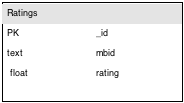
\includegraphics[scale=1]{DatabaseScheme.png} \\
	De lokale database moet data bijhouden die offline geraadpleegd zou willen worden. Hierbij reken ik op een geschiedenis van de laatste zoekopdrachten, bekeken liedjes en de laatst gegeven scores. Aangezien deze applicatie vooral beroep doet op een actieve internetverbinding, zal er niet veel meer dan dat opgeslagen worden. \\
	 De implementatie van deze database gebeurt in SQLite.
	 
	 \begin{itemize}
		\item Ratings table \newline
		\begin{tabular}{| l | l | l | }
		\hline
		id & integer & primary key \\
		date & date & \\
		rating & float & \\
		mbid & text & \\
		title & text & \\
		artist & text & \\
		\hline
		\end{tabular}
		
	\small \textit{Tabel \tabID : Het model van de Rating tabel in de lokale database.} \\ \normalsize
	
	%todo _id, name, title, mbid, date, rating
		\item Geschiedenis table \newline
		\begin{tabular}{| l | l | l | }
		\hline
		 id & integer & primary key \\
		date & date & \\
		rating & float & \\
		mbid & text & \\
		title & text & \\
		artist & text & \\
		\hline
		\end{tabular}
	
	\small \textit{Tabel \tabID : De Geschiedenis tabel in de lokale database.} \\ \normalsize
	
	 \end{itemize}
	

	\subsubsection{Externe Database}
	De externe database moet enkel scores van gebruikers verzamelen. Om verschillende gebruikers te identificeren zal de Android device ID mee opgeslagen worden. De tabel zal er dan zo uitzien: \\ \newline
		\begin{tabular}{| l | l | l | }
		\hline
		 id & integer & primary key \\
		date & date & \\
		rating & float & \\
		mbid & text & \\
		title & text & \\
		artist & text & \\
		userID & text & \\
		\hline
		\end{tabular}
	
	\small \textit{Tabel \tabID : De Rating tabel layout van de database op de server.} \\ \normalsize
		
%\section{Vereisten en voortgang}
%Voor de voortgang van dit project besproken wordt, eerst een opsomming van alle vereisten en huidige status. \\
%
%	\begin{tabular}{| c | p{\linewidth} | }
%	\hline
%	Datum & Informatie \\ \hline \hline 
%	24-10 & Informatie ontvangen i.v.m. opdracht \\ \hline
%	07-11 & Afspraak met begeleiders en promoter, acceptatie bachelorproef \\ \hline
%	21-11 & Android project aangemaakt met simpele GUI. Ook Last.fm account aangemaakt en unieke API sleutel aangevraagd. \\ \hline
%	05-12 & Gebruikers kunnen echte calls maken en muziek opzoeken. Zitten nog bugs in en er kan nog niet gezocht worden naar artiesten \\ \hline
%	19-12 & Er kan ook gezocht worden op artiesten, GUI werd herzien, abstractie in code toegevoegd. \\ \hline
%	03-01 & Een score kan worden opgeslagen in de lokale database, en het totaal en gemiddelde kan uitgelezen worden. \\ \hline
%	xx-xx & Todo: Titel en artiest mee opslagen voor geschiedenis GUI. Ook nog op artiest kunnen zoeken. \\ \hline
%	
%	\end{tabular} \\ 
%	\small \textit{Tabel \tabID : Enkele belangrijke highlights in de voortgang van het project.} \newline \normalsize
%	
%
%Zoals in de sectie Vereisten gezien kan worden, is de applicatie langs de client-kant haast volledig af. Men kan al muziek nummers opzoeken, selecteren en beoordelingen geven die effectievelijk opgeslagen worden in een database. Wat er momenteel aan deze kant nog ontbreekt is een manier om enkel op artiest te zoeken en gebruik geschiedenis te kunnen bekijken. \\
%Nadat deze twee zaken geïmplementeerd zijn, is de applicatie langs de client-side af. Dan moet er aan de server side gewerkt worden. Dit houdt in dat scores naar de data-collection server gestuurd moeten worden, en occassioneel scores gedownloaded moeten kunnen worden. \\
	
	
	
\newpage % hack for layout	
	%%%%%%%%%%%%%%%
	% GUI SECTION %
	%%%%%%%%%%%%%%%
\section{GUI}
	Hieronder volgen enkele schermopnames van de voorlopige GUI. Deze zal normaal gezien niet veel meer veranderen naar het verloop van de rest van het project, maar men kan nooit zeker weten.\\
	Voor een voorbeeld van de huidige GUI volgt hier een voorbeeld van een gebruiker die de applicatie opstart en een lied opzoekt.  \\ \newline
	
	\begin{tabular}{l l}
		\begin{minipage}{5cm}
			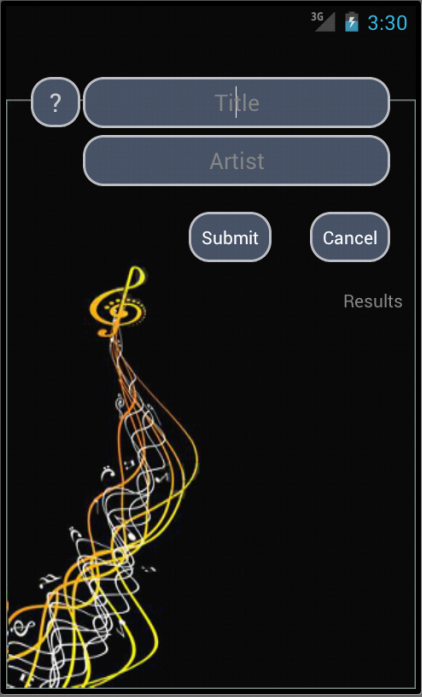
\includegraphics[scale=0.4]{GUI_0124_startscreen.png}
			\small \textit{Afbeelding \figID : Start scherm.} \\ \normalsize
		\end{minipage}
	%&
		\begin{minipage}{7cm}
			Dit scherm is het start scherm en het eerste wat de gebruiker ziet wanneer de applicatie gestart wordt. Er zijn twee velden om zoektermen in te geven (een voor artiest en een voor titel). De linkerboven knop met het vraagteken erop toont de instructies van de applicatie. De submit knop start een zoekopdracht, wanneer er zoektermen opgegeven zijn. De cancel knop wist alle ingevulde gegevens (zodat een andere zoekopdracht sneller uitgevoerd kan worden.)
		\end{minipage}
	\end{tabular} \\ \newline
	
	
	% Zoek- en downloadproces &
	\begin{tabular}{ p{8cm}  l }	
		\begin{minipage}{7cm}
			In het naaststaande scherm werden de zoektermen "Bohemian Rhapsody" en "Queen" ingevuld, en op de knop Submit geklikt. De applicatie heeft de zoektermen verwerkt en start het informatie download proces. De text "Loading..." verschijnt op het scherm om de gebruiker te laten weten dat de applicatie ermee bezig is. 
		\end{minipage}
		&
		\begin{minipage}{5cm}
			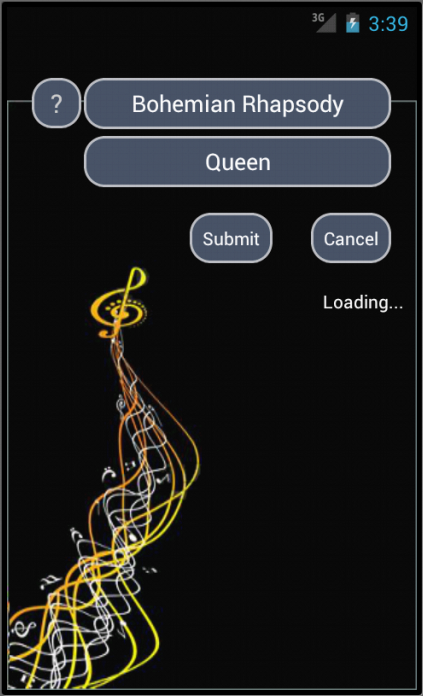
\includegraphics[scale=0.4]{GUI_0124_startsearch.png} 
			\small \textit{Afbeelding \figID : Zoek- en downloadproces.} \\ \normalsize
		\end{minipage}
	\end{tabular} \\ \newline
	
	
	%Klaar met downloaden \\	
	\begin{tabular}{ l  p{8cm} }
		\begin{minipage}{5cm}
			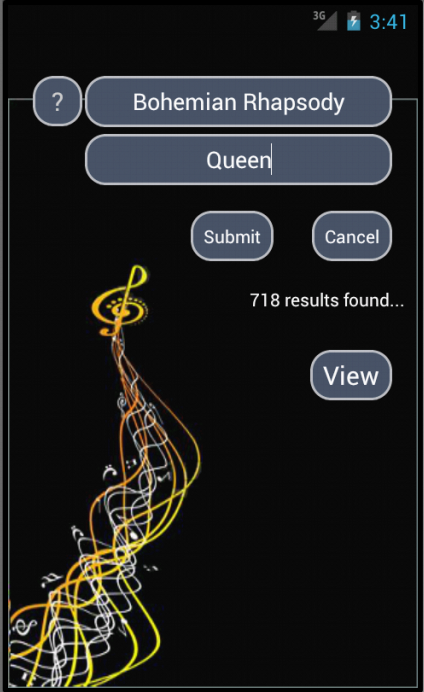
\includegraphics[scale=0.4]{GUI_0124_startresults.png}
			\small \textit{Afbeelding \figID : Klaar met downloaden.} \\ \normalsize
		\end{minipage}	
		
		\begin{minipage}{7cm}
			Wanneer de applicatie klaar is met het antwoord van de server te downloaden, verandert de text "Loading..." in het resultaat van de oproep, en het aantal gevonden resultaten. Wanneer er een positief aantal resultaten gevonden werd, verschijnt de knop View, waar de gebruiker op kan klikken om de resultaten te bekijken en het gewenste item te selecteren.
		\end{minipage}
	\end{tabular} \\ \newline


	% Geeft alle resultaten weer &
	\begin{tabular}{ p{8cm}  l }
		\begin{minipage}{7cm}
			De lijst die resultaten weergeeft. Men kan op elke optie klikken om naar een pagina te gaan met meer informatie. Opties die niet beschikken over een afbeelding krijgen de standaard "Niet beschikbaar" afbeelding. De anderen worden asynchroon gedownloaded.
		\end{minipage}
		&
		\begin{minipage}{5cm}
			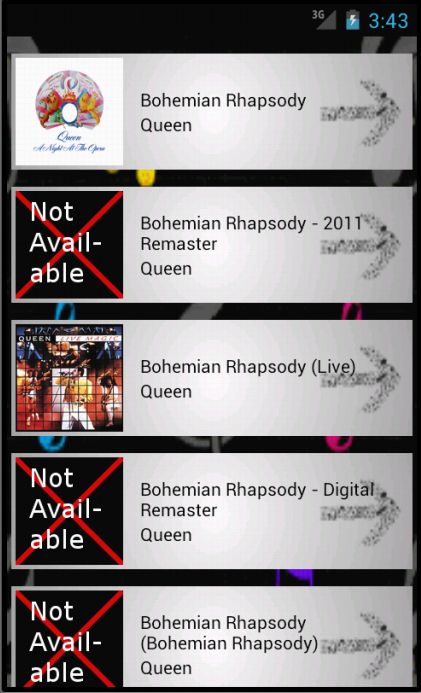
\includegraphics[scale=0.4]{GUI_0124_results.png} 
			\small \textit{Afbeelding \figID : Lijst met zoekresultaten.} \\ \normalsize
		\end{minipage}
	\end{tabular} \\ \newline
	
	
	% Weergave van een track \\
	\begin{tabular}{ l  p{8cm} }
		\begin{minipage}{5cm}
			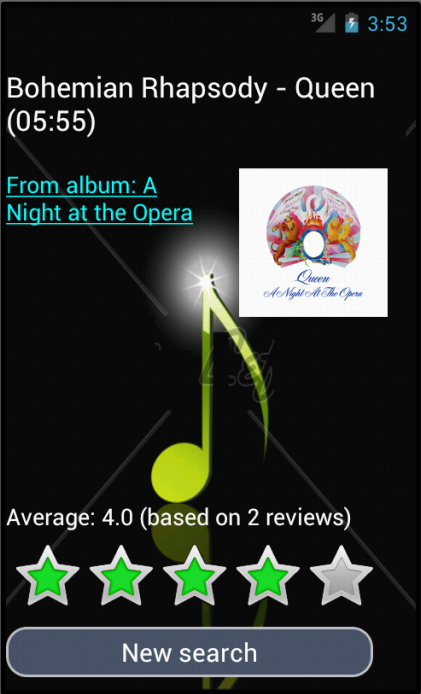
\includegraphics[scale=0.4]{GUI_0124_track.png} 
			\small \textit{Afbeelding \figID : Gedetailleerd scherm voor een lied.} \\ \normalsize
		\end{minipage}
		
		\begin{minipage}{7cm}
			Dit scherm geeft de gedetailleerde pagina van een individueel lied weer. De duratie van het lied wordt getoond, het album van het lied, een afbeelding en het score systeem. Het gemiddelde en het aantal van alle stemmen voor dat lied wordt getoond, en 5 sterren bieden de mogelijkheid aan de gebruiker om een eigen score aan het lied toe te dienen. Helemaal onderaan de knop om een nieuwe zoekopdracht te starten.
		\end{minipage}
	\end{tabular} \\ \newline
	
	
	% Albumscherm &
	\begin{tabular}{ p{8cm}  l }
		\begin{minipage}{7cm}
			Wanneer er meer album informatie beschikbaar is en de gebruiker klikt op het album, komt hij op dit scherm terecht. Het bevat informatie over een gegeven album zoals artiest, albumafbeelding, playcount, listeners, een scrollbare album informatie tekst en alle liedjes die op dat album staan. De gebruiker kan op elk lied klikken om naar de gedetailleerde liedjes pagina te gaan. 
		\end{minipage}
		&
		\begin{minipage}{5cm}
			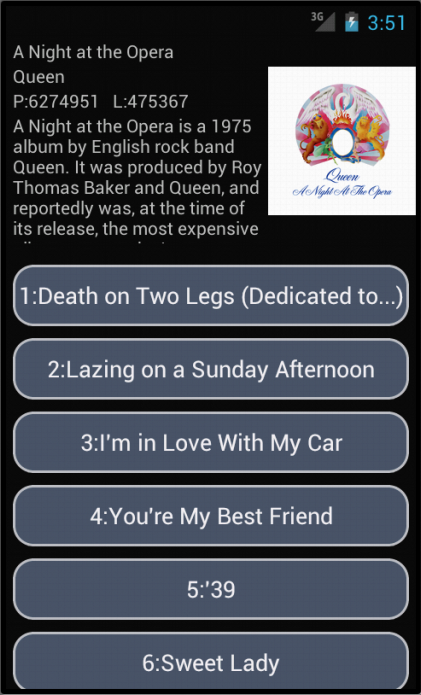
\includegraphics[scale=0.4]{GUI_0124_album.png} 
			\small \textit{Afbeelding \figID : Gedetailleerd scherm voor een album.} \\ \normalsize
		\end{minipage}
	\end{tabular}
			
	

\section{Problemen}
	\subsection{Synchronious tasks}
	Wanneer data binnengehaald moet worden van de API, mag die operatie niet gebeuren op de main thread van het programma, anders zal de applicatie zeer traag/onbruikbaar zijn elke keer dat er iets gedownloaded moet worden. Hierom werd een klasse "MyConnection" gemaakt, die async\footnote{Asynchronous betekent dat een process tegelijkertijd naast een ander process kan werken.} data begint binnen te laden terwijl de applicatie vloeiend kan blijven voortdraaien.
	\subsection{Tracks omzetten van verschillende representaties}
	Een tegengekomen probleem in dit project, is dat de Last.fm API oproepen (zoals track.getinfo en track.search) antwoorden met verschillende representaties. Om een voorbeeld te geven: hieronder bevinden zich de resultaten van twee oproepen naar methoden voor het lied 'Bohemian Rhapsody' van Queen. Er kan opgemerkt worden dat in het eerste resultaat 'artist' een top level attribuut is van 'track'. In het tweede snippet is 'artist' opnieuw een object met zijn eigen velden. Om zo een object\footnote{In dit document gebruik ik XML notatie omdat deze makkelijker leesbaar is, maar in de broncode wordt er enkel met JSON gewerkt.} om te zetten in een 'Track' klasse, moet de Track klasse een onderscheid maken in wat voor soort object gebruikt wordt om de klasse te initialiseren. De beste oplossing hiervoor is om per representatie een loadFromX functie te maken die weet hoe X eruit ziet en waar alle informatie staat. \\
	
	Track.search resultaat:\\
	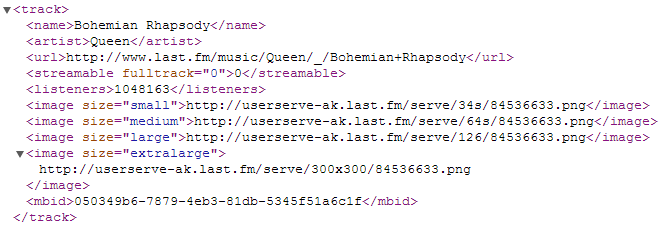
\includegraphics[width=15cm]{track_search.png} \\ \newline
	\small \textit{Afbeelding \figID : Resultaat van Track.search GET voor Bohemian Rhapsody - Queen.} \\

	Track.getinfo resultaat: \\
	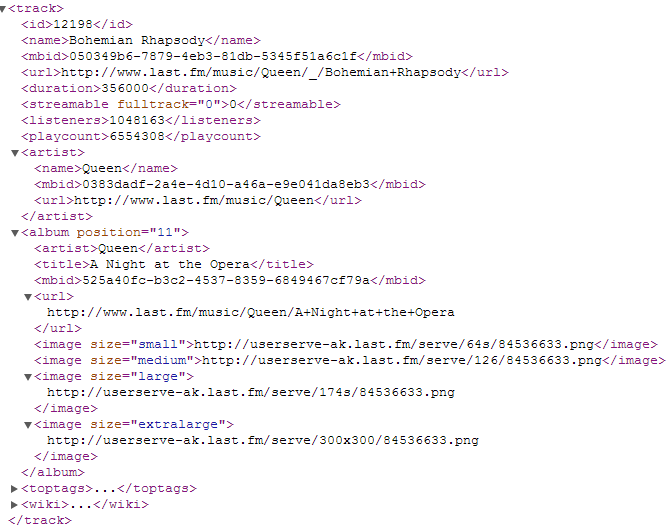
\includegraphics[width=15cm]{track_getinfo.png}\\ \newline
	\small \textit{Afbeelding \figID : Resultaat van Track.getinfo GET voor Bohemian Rhapsody - Queen.}
		


	
	
\section{Bronnen, tools en referenties}

	\begin{itemize}
			
	\item \textbf{Eclipse} \\
	Programmeerplatform Eclipse (Juno) werd gebruikt voor de implementatie en emulatie.	\\
	\url{http://www.eclipse.org/}

	\item \textbf{Android Development Toolkit (ADT)} \\
	Deze plug-in bevat alle benodigdheden om programma's voor Android in Eclipse te bouwen en testen.\\
	\url{http://developer.android.com/sdk/index.html}

	\item \textbf{AMuRate homepagina} \\
		\url{http://dsverdlo.github.com/AMuRate}
		
	\item \textbf{Android} \\
		\url{http://www.android.com/}
		
	\item \textbf{Ice Cream Sandwich} \\
		\url{http://www.android.com/about/ice-cream-sandwich/}	
		
	\item \textbf{Last.fm} \\
		\url{http://www.last.fm/home}	
		
	\item \textbf{Github} \\
		\url{https://github.com/}



	\end{itemize}



\end{document}
